\documentclass[11pt, oneside, a4paper]{report}
\usepackage{cite}
\usepackage[british]{babel}
\usepackage{import}
\usepackage{setspace}

% \usepackage{appendix}
\usepackage[bottom]{footmisc}
\usepackage{siunitx} % Provides the \SI{}{} and \si{} command for typesetting SI units
\usepackage{graphicx} % Required for the inclusion of images
\usepackage[table,xcdraw]{xcolor}
\usepackage{natbib} % Required to change bibliography style to APA
\newcommand*{\urlprefix}{Available from: }
\newcommand*{\urldateprefix}{Accessed }
\bibliographystyle{bath}   
\usepackage{amsmath} % Required for some math elements
\usepackage{mathtools}
\usepackage{caption}
\usepackage[none]{hyphenat}
\setlength\parindent{0pt} % Removes all indentation from paragraphs
\usepackage{lscape}
\usepackage[super]{nth}
\usepackage{float}
\usepackage{times}
\usepackage[a4paper, margin=1in]{geometry}
% \usepackage{subfig}
\usepackage{subcaption}
\newcommand*{\transpose}{\mathrm{T}}
\newcommand*{\vc}[1]{\mathbf{#1}}
\usepackage{listings}
\usepackage{pdfpages}
\usepackage{fancyhdr}
\usepackage[T1]{fontenc}
\usepackage{wrapfig}
\usepackage{longtable}
\usepackage{enumerate}
\usepackage{titlepic}
\usepackage{listings}
\usepackage{python}
\usepackage{helvet}
\usepackage{multicol}
% \usepackage[framed,numbered,autolinebreaks,useliterate]{mcode}
\pagestyle{empty}
\usepackage{minted}
\usepackage[hidelinks]{hyperref}
\usepackage{python}
% \renewcommand{\thefigure}{\arabic{section}.\arabic{figure}}
% \renewcommand{\theequation}{\arabic{section}.\arabic{equation}}
% \renewcommand{\thetable}{\arabic{section}.\arabic{table}}
\fancyhead[LE,RO]{Final Report}
\fancyhead[RE,LO]{XX40197}
\fancyfoot[CE,CO]{}
\fancyfoot[LE,RO]{\thepage}
\renewcommand{\footrulewidth}{1pt}
\renewcommand{\thefigure}{\arabic{chapter}.\arabic{figure}}
\renewcommand{\theequation}{\arabic{chapter}.\arabic{equation}}
\renewcommand{\thetable}{\arabic{chapter}.\arabic{table}}
\renewcommand{\thelisting}{\arabic{chapter}.\arabic{listing}}

\fancypagestyle{plain}{%
  \fancyhf{}%
  \fancyfoot[R]{\thepage}%
  \renewcommand{\headrulewidth}{0pt}% Line at the header invisible
  \renewcommand{\footrulewidth}{0.4pt}% Line at the footer visible
}

\definecolor{codegreen}{rgb}{0,0.6,0}
\definecolor{codegray}{rgb}{0.5,0.5,0.5}
\definecolor{codepurple}{rgb}{0.58,0,0.82}
\definecolor{backcolour}{rgb}{0.95,0.95,0.92}
\lstdefinestyle{mystyle}{
    backgroundcolor=\color{backcolour},  
    commentstyle=\color{codegreen},
    keywordstyle=\color{magenta},
    numberstyle=\tiny\color{codegray},
    stringstyle=\color{codepurple},
    basicstyle=\ttfamily\footnotesize,
    breakatwhitespace=false,        
    breaklines=true,                
    captionpos=b,                    
    keepspaces=true,                
    numbers=left,                    
    numbersep=5pt,                  
    showspaces=false,                
    showstringspaces=false,
    showtabs=false,                  
    tabsize=2
}
\lstset{style=mystyle}


\begin{document}
\begin{titlepage}
    \title{"Submarine Communication during Lightning Interference"\\ Final Year Project \\ XX40197}
    % \titlepic{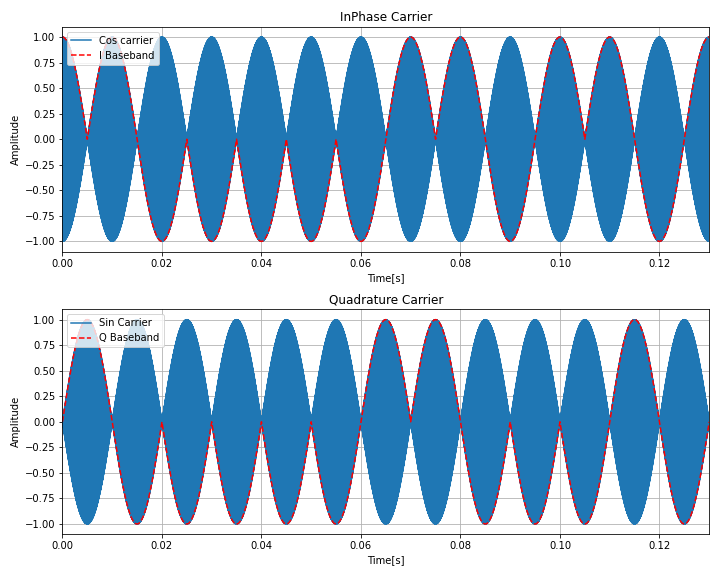
\includegraphics[width=0.5\textwidth]{figs/sim/carrier.png}}
    \author{Candidate 13220
    \\[0.5cm]
    Supervisor: Martin Fullerkrug
    \\[0.5cm] 
    Assessor: Nigel Johnston}
    \date{\textit{May 2021}}
\end{titlepage}



\maketitle

\import{Sections/}{summary.tex}

\pagestyle{empty}
\tableofcontents

\newpage
\pagenumbering{roman}
\renewcommand{\thesection}{\Roman{section}}
\addcontentsline{toc}{section}{List of Figures}
\listoffigures
\pagestyle{fancy}
\pagebreak
\addcontentsline{toc}{section}{List of Tables}
\listoftables
\pagebreak

\import{Sections/}{list_of_symbols.tex}
\newpage
\setcounter{section}{0}

\pagenumbering{arabic}
\setcounter{page}{1}
\renewcommand{\thesection}{\arabic{chapter}.\arabic{section}}
% \setstretch{1.25}
\import{Sections/}{Introduction.tex}
\pagebreak
\import{Sections/}{LitReview.tex}
\pagebreak
\import{Sections/}{methods.tex}
\pagebreak
\import{Sections/}{results.tex}
\pagebreak
\import{Sections/}{discussion.tex}
\pagebreak
\import{Sections/}{conclusions.tex}
\renewcommand{\bibname}{References}
% \setstretch{1.0}
\addcontentsline{toc}{chapter}{References}
\bibliography{refs}
% \appendix
% \addcontentsline{toc}{chapter}{Appendices}
% \import{Sections/Appendices/}{AppendixA.tex}
% \import{Sections/Appendices/}{AppendixB.tex}
% \import{Sections/Appendices/}{AppendixC.tex}
\end{document}